%%%%%%%%%%%%%%%%%%%%%%%%%%%%%%%%%%%%%%%%%
% Beamer Presentation
% LaTeX Template
% Version 1.0 (10/11/12)
%
% This template has been downloaded from:
% http://www.LaTeXTemplates.com
%
% License:
% CC BY-NC-SA 3.0 (http://creativecommons.org/licenses/by-nc-sa/3.0/)
%
%%%%%%%%%%%%%%%%%%%%%%%%%%%%%%%%%%%%%%%%%

%----------------------------------------------------------------------------------------
%	PACKAGES AND THEMES
%----------------------------------------------------------------------------------------

%\documentclass[aspectratio=169]{beamer}
\documentclass{beamer}

\mode<presentation> {

% The Beamer class comes with a number of default slide themes
% which change the colors and layouts of slides. Below this is a list
% of all the themes, uncomment each in turn to see what they look like.

%\usetheme{default}
%\usetheme{AnnArbor}
%\usetheme{Antibes}
%\usetheme{Bergen}
%\usetheme{Berkeley}
%\usetheme{Berlin}
%\usetheme{Boadilla}
%\usetheme{CambridgeUS}
%\usetheme{Copenhagen}
%\usetheme{Darmstadt}
%\usetheme{Dresden}
%\usetheme{Frankfurt}
%\usetheme{Goettingen}
%\usetheme{Hannover}
%\usetheme{Ilmenau}
%\usetheme{JuanLesPins}
%\usetheme{Luebeck}
\usetheme{Madrid}
%\usetheme{Malmoe}
%\usetheme{Marburg}
%\usetheme{Montpellier}
%\usetheme{PaloAlto}
%\usetheme{Pittsburgh}
%\usetheme{Rochester}
%\usetheme{Singapore}
%\usetheme{Szeged}
%\usetheme{Warsaw}

% As well as themes, the Beamer class has a number of color themes
% for any slide theme. Uncomment each of these in turn to see how it
% changes the colors of your current slide theme.

%\usecolortheme{albatross}
%\usecolortheme{beaver}
%\usecolortheme{beetle}
%\usecolortheme{crane}
%\usecolortheme{dolphin}
%\usecolortheme{dove}
%\usecolortheme{fly}
%\usecolortheme{lily}
%\usecolortheme{orchid}
%\usecolortheme{rose}
%\usecolortheme{seagull}
%\usecolortheme{seahorse}
%\usecolortheme{whale}
%\usecolortheme{wolverine}

%\setbeamertemplate{footline} % To remove the footer line in all slides uncomment this line
%\setbeamertemplate{footline}[page number] % To replace the footer line in all slides with a simple slide count uncomment this line

%\setbeamertemplate{navigation symbols}{} % To remove the navigation symbols from the bottom of all slides uncomment this line
}

\usepackage{graphicx} % Allows including images
\usepackage{booktabs} % Allows the use of \toprule, \midrule and \bottomrule in tables
\usepackage{color, colortbl}
\usepackage{graphicx}
%\usepackage[lined]{algorithm2e}
\usepackage[ruled,vlined]{algorithm2e}
%\usepackage{beamerthemesplit}
%----------------------------------------------------------------------------------------



%	TITLE PAGE
%----------------------------------------------------------------------------------------

%\title[Six Algorithms]{Six Algorithms \\ \footnotesize Select Typical Machine Learning Algorithms for Data Analytics} % The short title appears at the bottom of every slide, the full title is only on the title page

\title[Distributed GBT]{HARP DAAL Update}
\subtitle{Distributed Gradient Boosting Tree}

\author{Bo Peng} % Your name
\institute[IUB] % Your institution as it will appear on the bottom of every slide, may be shorthand to save space
{
Digital Science Center \\
Indiana University\\ % Your institution for the title page
\medskip
\textit{pengb@indiana.edu} % Your email address
}
\date{\today} % Date, can be changed to a custom date

\begin{document}
	

%----------------------------------------------------------------------------------------
%	PRESENTATION SLIDES
%----------------------------------------------------------------------------------------
\begin{frame}
	\maketitle
\end{frame}

\AtBeginSubsection[]
{
	\begin{frame}
		\frametitle{Outline} % Table of contents slide, comment this block out to remove it
		\tableofcontents[currentsection,currentsubsection, 
		sectionstyle=show/shaded,
		] % Throughout your presentation, if you choose to use \section{} and \subsection{} commands, these will automatically be printed on this slide as an overview of your presentation
	\end{frame}
} 
%------------------------------------------------
\section{Background} % Sections 
\subsection{GBT Algorithm} 
\begin{frame}
	\frametitle{Regression}
	\begin{columns}[c] % The "c" option specifies centered vertical alignment while the "t" option is used for top vertical alignment
		
		\column{.45\textwidth} % Left column and width
		%\textbf{Heading}
		\begin{figure}
			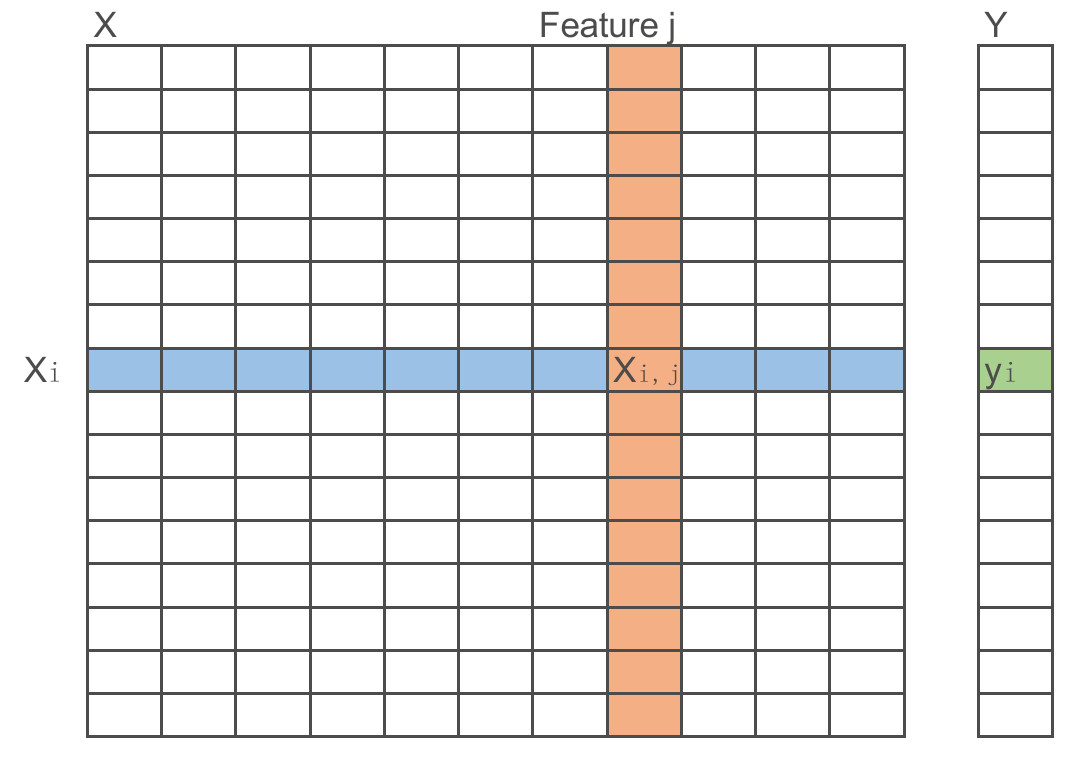
\includegraphics[width=1\linewidth]{figs/dataset.jpg}
		\end{figure}
		
		\column{.5\textwidth} % Right column and width
		\begin{itemize}
			\item Problem: find $\widehat{y_i}=\phi(x_i)$ that minimize regularized objective
			$\mathcal{L(\phi)}= \sum_{i=1}^{n}{\ell{(\widehat{y_i},y_i}) + \Omega(\phi)}$

			\item Loss function, for example $\ell{(\widehat{y_i},y_i})=(\widehat{y_i}-y_i)^2$
			\item Data: \\
			Input: $n$ samples $x_i$ each as a $m$ dimensional vector, \\
			Response: $n$ responses $y_i$
		\end{itemize}
	\end{columns}	
\end{frame}

\begin{frame}
	\frametitle{Regression Tree}
		\begin{figure}
			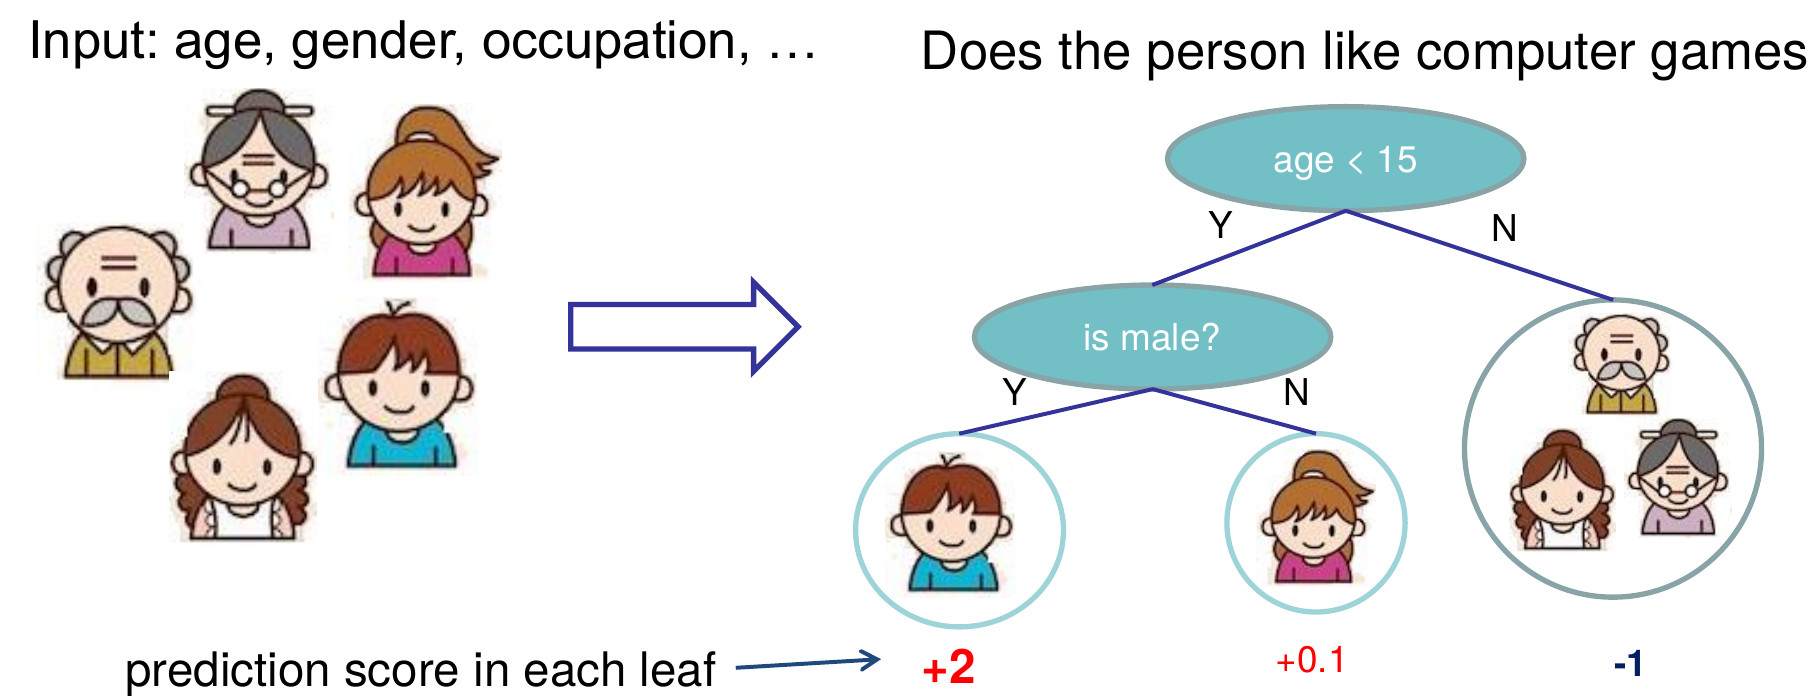
\includegraphics[width=1\linewidth]{figs/regressiontree}
		\end{figure}
		
		\begin{itemize}
			\item Regression Tree: $f(x)=w_{q(x)}$ where $q: \mathbb{R}^m \rightarrow T$\\ 
			$q$ is the tree structure, map $x$ to leaf nodes ($T$ is number of leaves) \\
			$w$ is leaf weights		
			\item How to learn $f(x)$ ? \\ 
			Greedy algorithm, \textcolor{red}{findBestSplit()} according to a \textcolor{red}{score function} at each internal node
			
		\end{itemize}
	
\end{frame}

\begin{frame}
	\frametitle{Boosting}
	\begin{figure}
		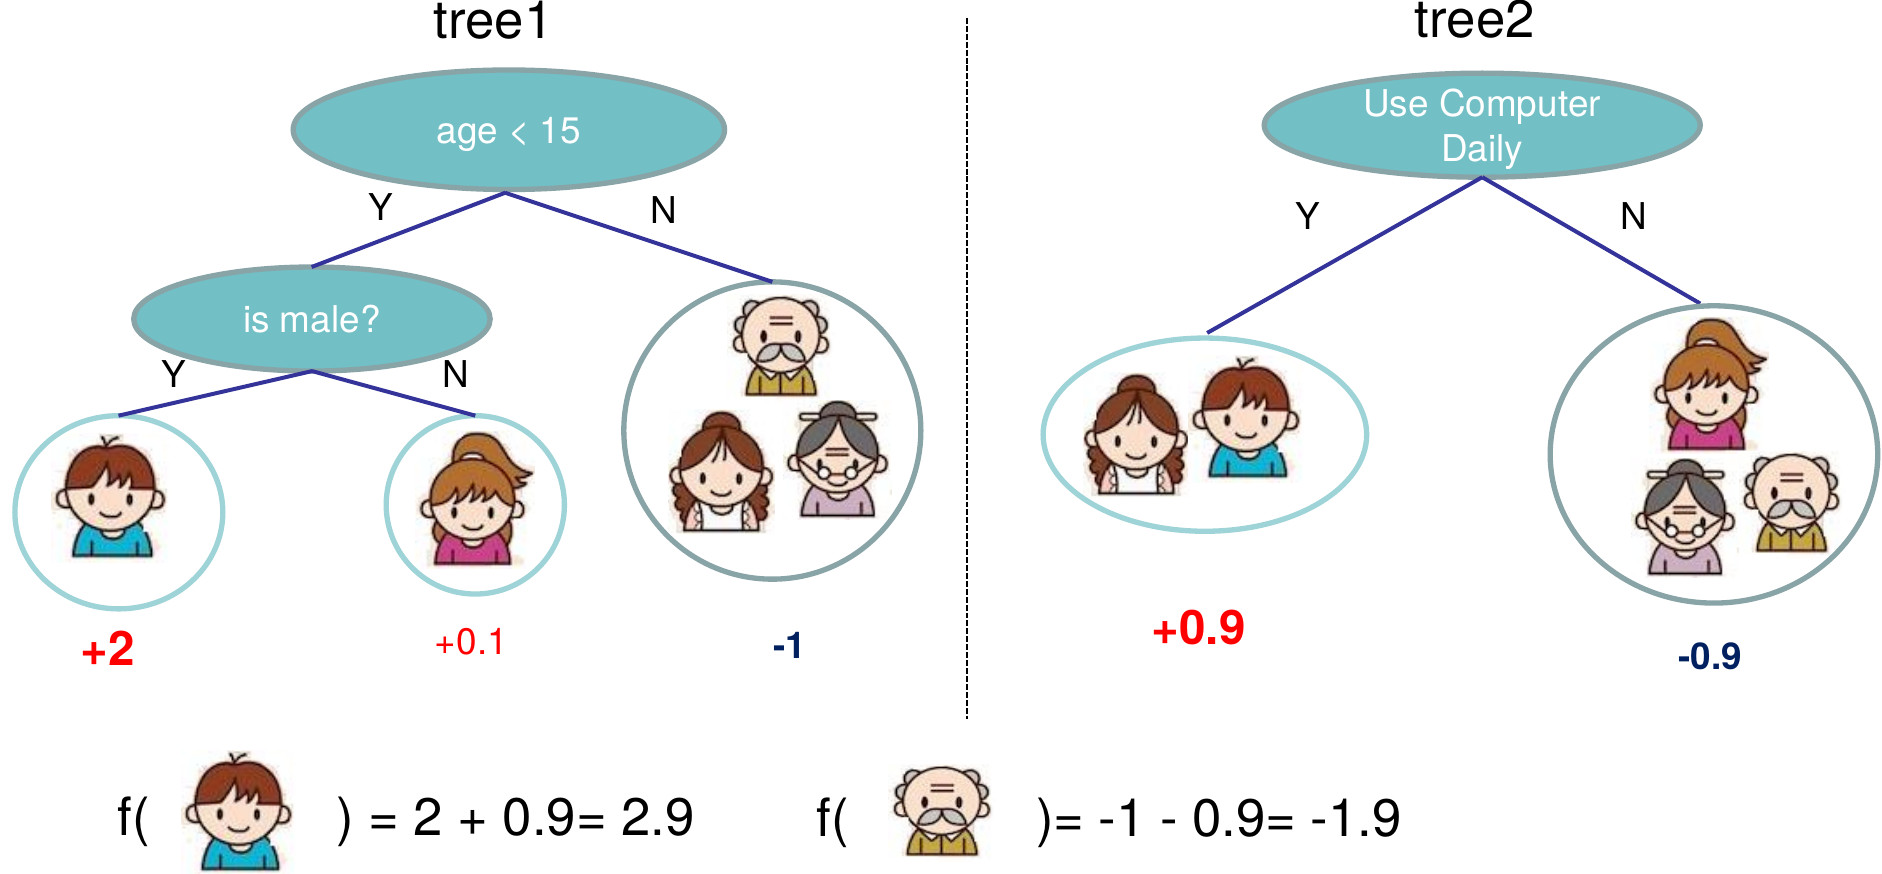
\includegraphics[width=1\linewidth]{figs/boostingtree}
	\end{figure}
	
	\begin{itemize}
		\item Boosting: $\widehat{y_i}=\phi(x_i)=\sum_{k=1}^{K}f_k(x_i)$  
		\item additive model: prediction is the sum score of all the trees
	\end{itemize}
	
\end{frame}

\begin{frame}
	\frametitle{GBT:Gradient Boosting Tree}
	\begin{itemize}
		\item \textcolor{red}{stage-wise} adding new tree: \\
		$\mathcal{L}^{(t)}= \sum_{i=1}^{n}{\ell{(\widehat{y}_i^{(t-1)}+f_t(x_i),y_i}) + \Omega(f_t)}$  
		\item by \textcolor{red}{second order approximation}
		$\mathcal{L}^{(t)}\approx \sum_{i=1}^{n}[{\ell{(\widehat{y}_i^{(t-1)},y_i}) + g_if_t(x_i)+\frac{1}{2}h_if_t^2(x_i)]+ \Omega(f_t)} $ \\
		where; \\
		$g_i = \partial_{\widehat{y}_i^{(t-1)}}{\ell(\widehat{y}_i^{(t-1)},y_i)}$ \\
		$h_i = \partial_{\widehat{y}_i^{(t-1)}}^2{\ell(\widehat{y}_i^{(t-1)},y_i)}$
		\item optimal weight $w_j^*$ and value for leaf $j$ should be \\
		$w_j^{*} = -\frac{\sum_{i \in I_j}g_i}{\sum_{i \in I_j}h_i +\lambda}$ \\
		$\widetilde{\mathcal{L}}^{(t)}= -\frac{1}{2}\sum_{j=1}^{T}{\frac{(\sum_{i \in I_j}g_i)^2}{\sum_{i \in I_j}h_i +\lambda}} + \gamma T$ 
		
	\end{itemize}
	
\end{frame}

\begin{frame}
	\frametitle{GBT Example}
	\begin{itemize}
		\item Example
			\begin{itemize}
				\item square loss:  $\ell{(\widehat{y_i},y_i})=(\widehat{y_i}-y_i)^2$ 
				$g_i = \partial_{\widehat{y}_i^{(t-1)}}{\ell(\widehat{y}_i^{(t-1)},y_i)}=2(\widehat{y}_i^{(t-1)} -y_i)$\\
				$h_i = 2$
				\item intuitively optimal weight $w_j^*$ is just a kind of \textcolor{red}{average residual}\\
				$w_j^{*} = -\frac{\sum_{i \in I_j}g_i}{\sum_{i \in I_j}h_i +\lambda} = \frac{2}{2+\lambda}\frac{(y_i-\widehat{y}_i^{(t-1)})}{|I_j|}$
			\end{itemize}				
		\item Important data structure on leaf $j$
			\begin{itemize}
				\item $G_j = \sum_{i \in I_j}g_i$
				\item $H_j = \sum_{i \in I_j}h_i$
				\item $S(L,R) = \frac{G_{I_L}^2}{H_{I_L}+\lambda} + \frac{G_{I_R}^2}{H_{I_R}+\lambda} $ score function to get best split(impurity,more general the loss reduction)
			\end{itemize}						
	\end{itemize}
\end{frame}

\begin{frame}
	\frametitle{GBT Algorithm}
	\begin{columns}[c] % The "c" option specifies centered vertical alignment while the "t" option is used for top vertical alignment
	
	\column{.5\textwidth} % Left column and width
		\scalebox{0.65}{%
			\begin{algorithm}[H]
				\caption{Gradient Boosted Regression Tree}
				\LinesNumbered
				\SetKwInOut{Input}{input}
				\SetKwInOut{Output}{output}
				\Input{dataset $D = {(x_i, y_i)}_{i=1}^{n}$, parameter $\lambda, \alpha, m$ }
				\Output{$m$ trees $f(x)=w_q(x)$ }			
				\Begin{				
					Initialize()	\\
					\For{t=1 to m}{ 
						\tcp{BuildTree($\{(x_i,y_i)\}$)}
						
						$(w,q) = \arg\min_{f_t}{\sum_{i=1}^{n}[{\ell{(\widehat{y}_i^{(t-1)}+ \alpha f_t(x_i),y_i})] + \Omega(f_t)}}$
						
						\tcp{additive update}
						$f_t(x) = f_{t-1}(x) + \alpha f_t(x)$
					}
				}
			\end{algorithm}
		}
	
	\column{.85\textwidth} % Right column and width
		\scalebox{0.65}{%
			\begin{algorithm}[H]
				\caption{Greedy Split Finding}
				\LinesNumbered
				\SetKwInOut{Input}{input}
				\SetKwInOut{Output}{output}
				\Input{I, instance set of current node; d, feature dimension}
				\Output{split at the position with max score }			
				\Begin{				
					$score = 0$
					
					$G = \sum_{i \in I}g_i$
					
					$H = \sum_{i \in I}h_i$ 
					
					\For{k = 1 to d}{ 
						$G_L = 0; H_L = 0$   
						
						\For{j in sorted(I, by $X_{jk}$)}{
							$G_L = G_L + g_j; H_L = H_L + h_j$ \\
							$G_R = G - G_L; H_R = H - H_L$	\\						
							$score = max(score,\frac{G_L^2}{H_L + \lambda} + \frac{G_R^2}{H_R + \lambda})$
						}
					}
				}
			\end{algorithm}
		}
	\end{columns}	

\end{frame}

\begin{frame}
	\frametitle{GBT Summary}
	\begin{itemize}
		\item basic idea on
		\begin{itemize}
			\item boosting; function approximation target on the residual (gradient in general)
			\item decision tree; weak learner easy to understand and build
		\end{itemize}
		\item a general framework
		\begin{itemize}
			\item supporting wide range of loss functions and regularizations
			\item the score function to build tree is derived from a wide range of objective functions
		\end{itemize}
		\item features
		\begin{itemize}
			\item auto feature selection (kind of)
			\item easy to deal with missing values, category values
		\end{itemize}		

		
	\end{itemize}
	
\end{frame}

\section{Parallel and Distributed Implementation} % Sections 
\subsection{I. Shared-Memory} 
\begin{frame}
	\frametitle{Parallelism in a Shared-Memory Setting}
	\begin{columns}[c] % The "c" option specifies centered vertical alignment while the "t" option is used for top vertical alignment
		\column{.45\textwidth} % Left column and width
		%\textbf{Heading}
		\begin{figure}
			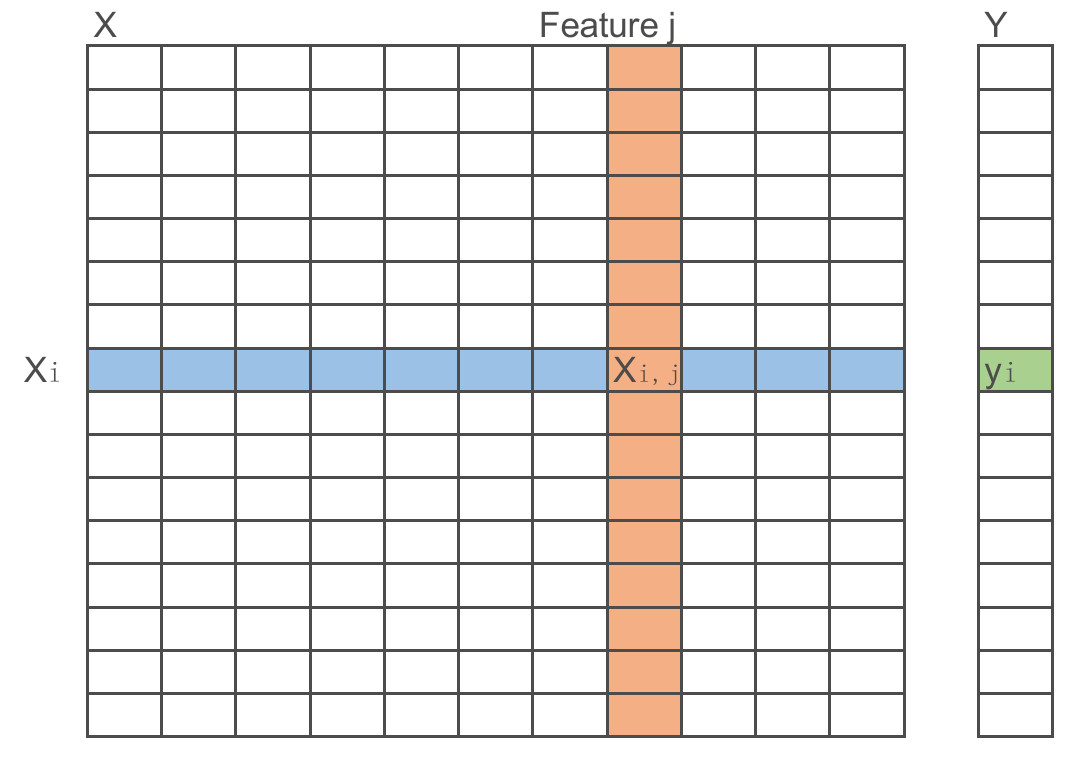
\includegraphics[width=1\linewidth]{figs/dataset.jpg} \\
			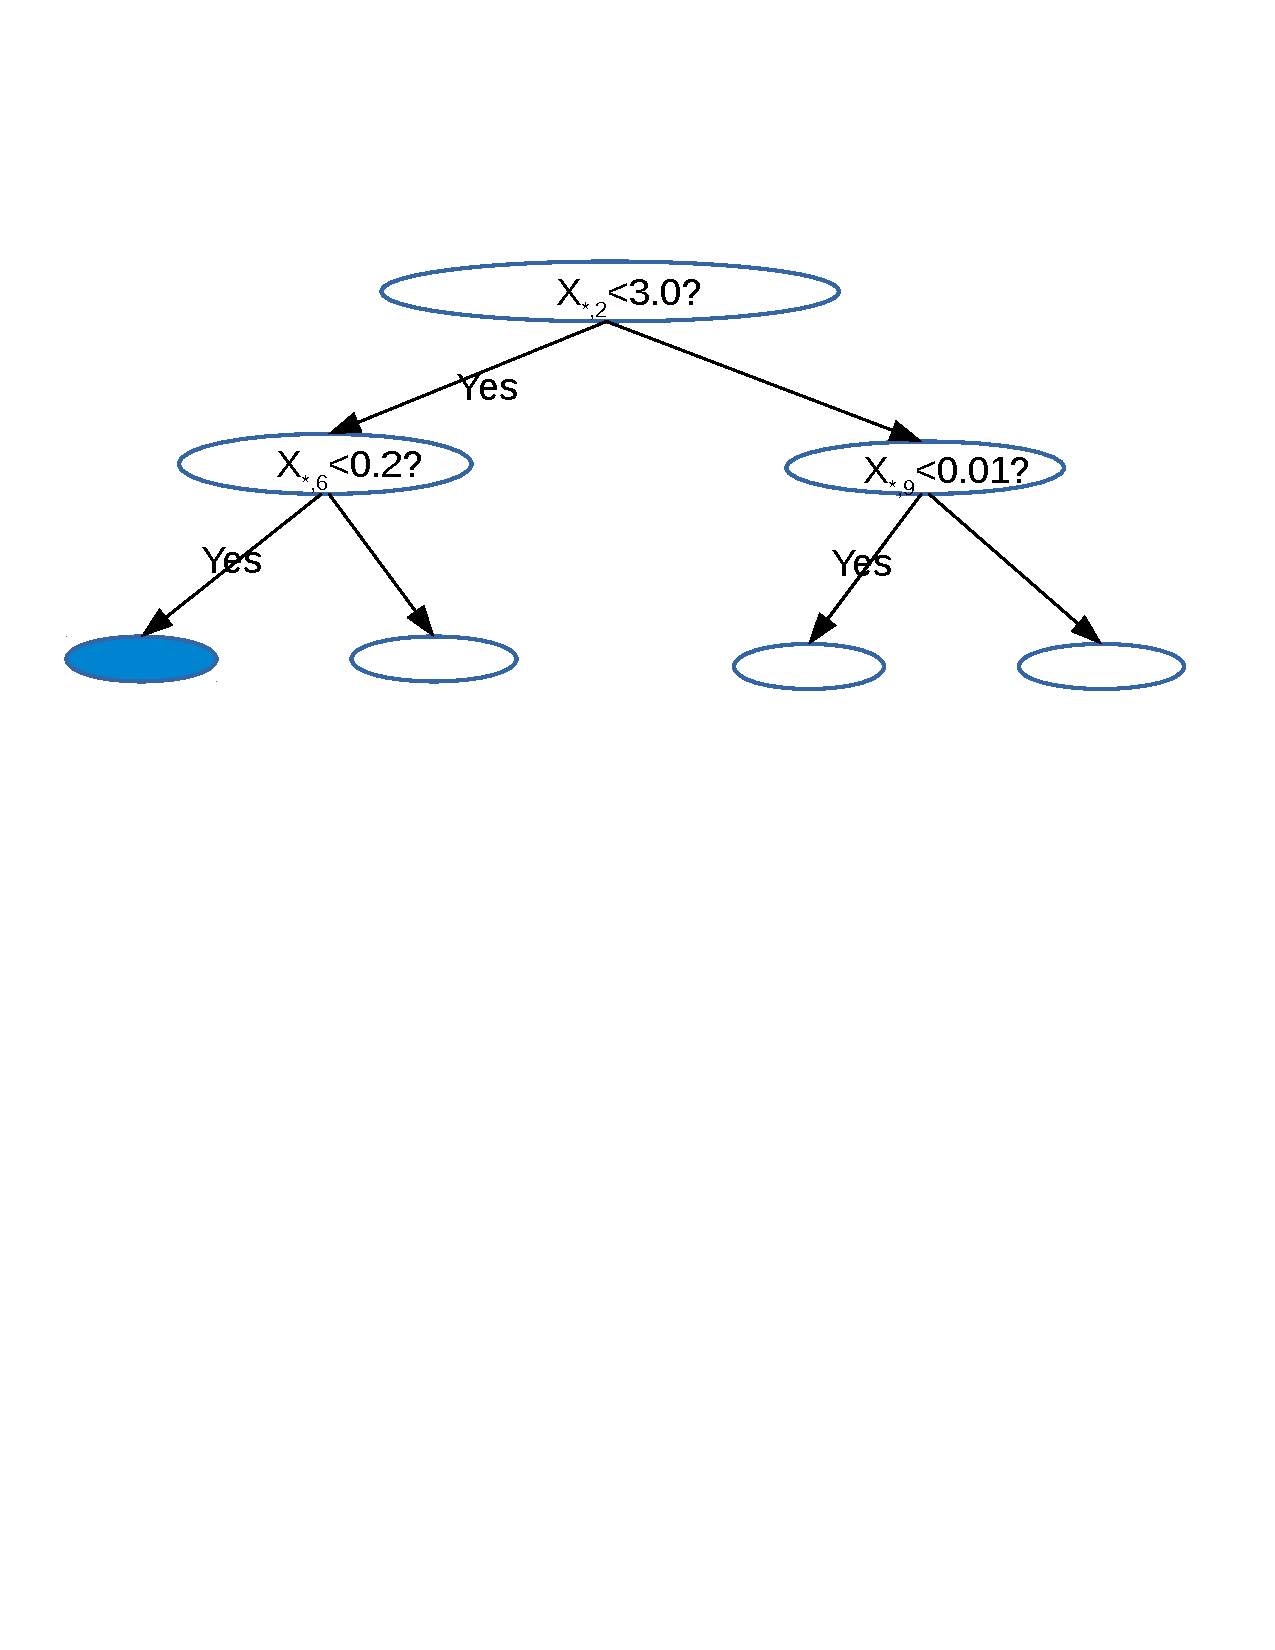
\includegraphics[width=1\linewidth]{figs/dtree}
		\end{figure}
		
		\column{.5\textwidth} % Right column and width
		\begin{itemize}
			\item Boosting is a sequential process, building trees one by one.(multiclass categorization have multiple boosting processes)
			\item Parallelism in building one tree
			\begin{itemize}			
				\item \textcolor{red}{parallelFeatures}: findBestSplit() works on features independently
				\item \textcolor{red}{parallelNodes}: same level of nodes in a tree works independently
				\item \textcolor{red}{vectorization}: lots of $\sum$ operations, $G_j, H_j$
			\end{itemize}			
		\end{itemize}
	\end{columns}	
\end{frame}

\begin{frame}
	\frametitle{Issues - Non-continous Mem Access}
	\begin{columns}[c] % The "c" option specifies centered vertical alignment while the "t" option is used for top vertical alignment
		\column{.7\textwidth} % Left column and width	
		\begin{figure}
			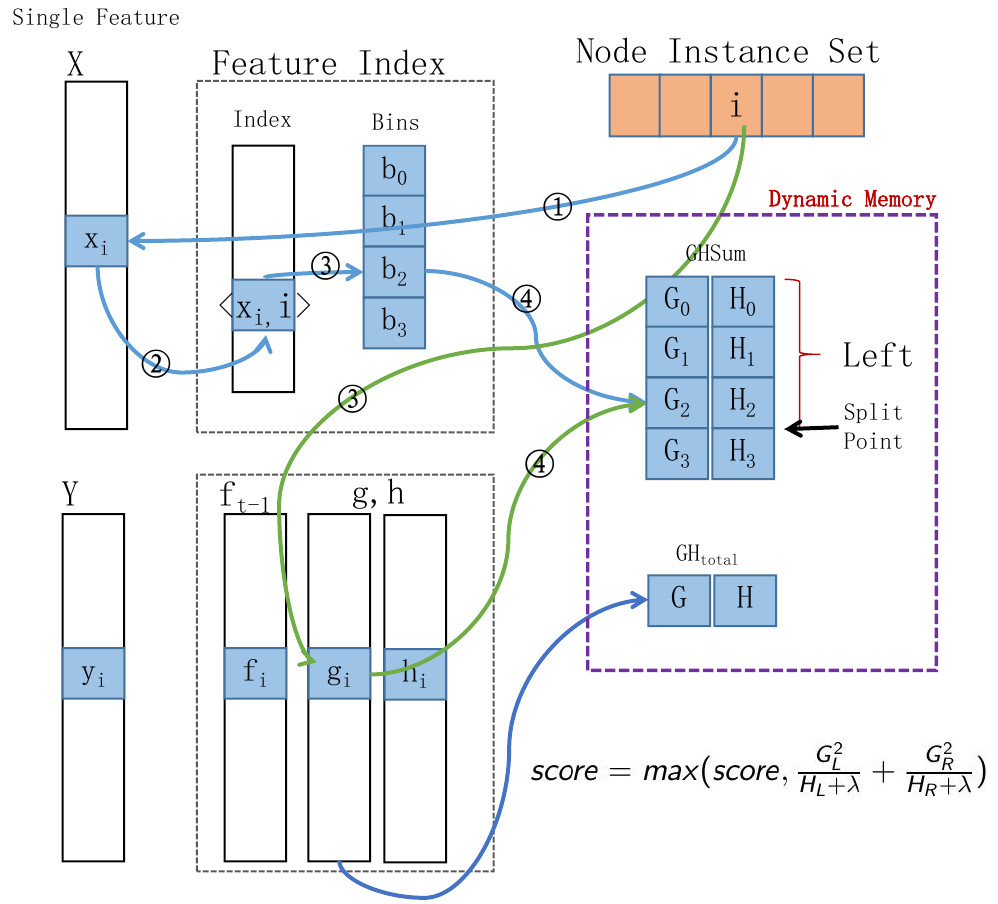
\includegraphics[width=1\linewidth]{figs/memaccess.jpg} 
		\end{figure}
		\column{.3\textwidth} % Right column and width
		\begin{itemize}
			\item \textcolor{red}{Bins} is a split candidates proposal $B={b_0,b_1,..,b_k}$, in general $|B| << n$
			\item with Bins, the findBestSplit timecomplexity drops from $\mathcal{O}(nlogn)$ to $\mathcal{O}(nlogb)$ 
		\end{itemize}
	\end{columns}		
\end{frame}


\subsection{II. Distributed} 
\begin{frame}
	\frametitle{Data Partition}
		%\textbf{Heading}
		\begin{figure}
			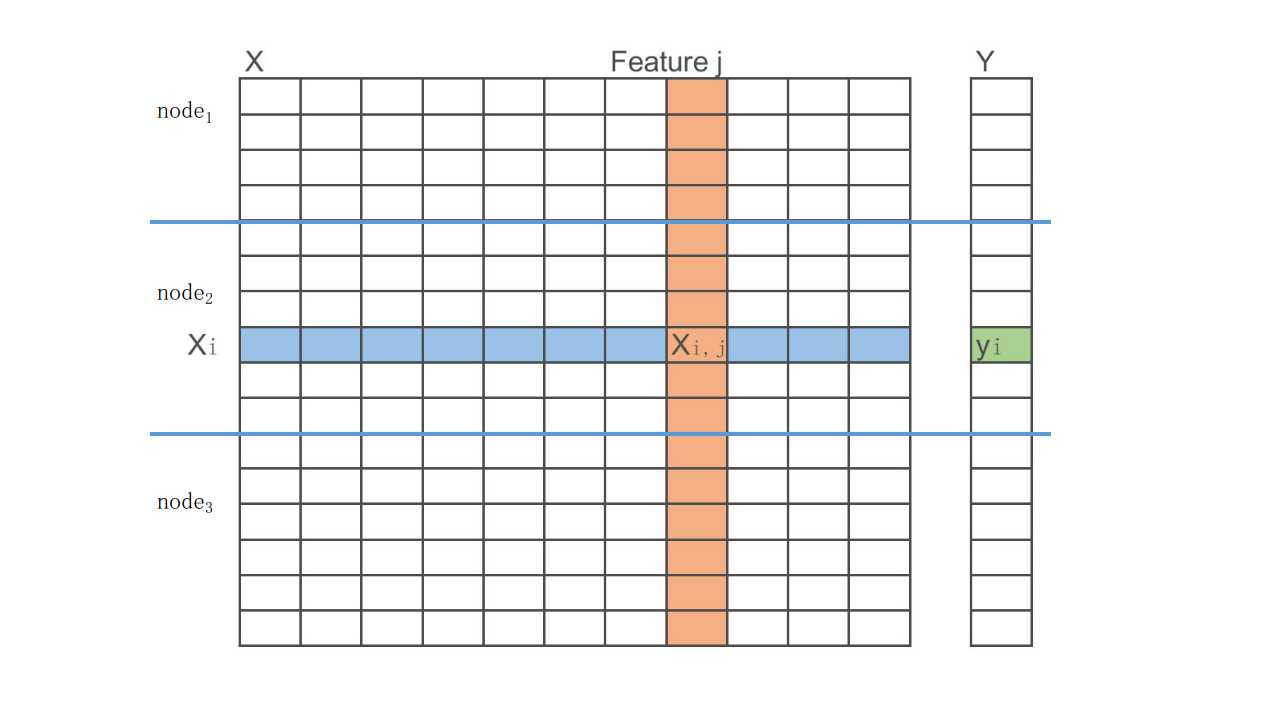
\includegraphics[width=.5\linewidth]{figs/datapartition1.jpg}
			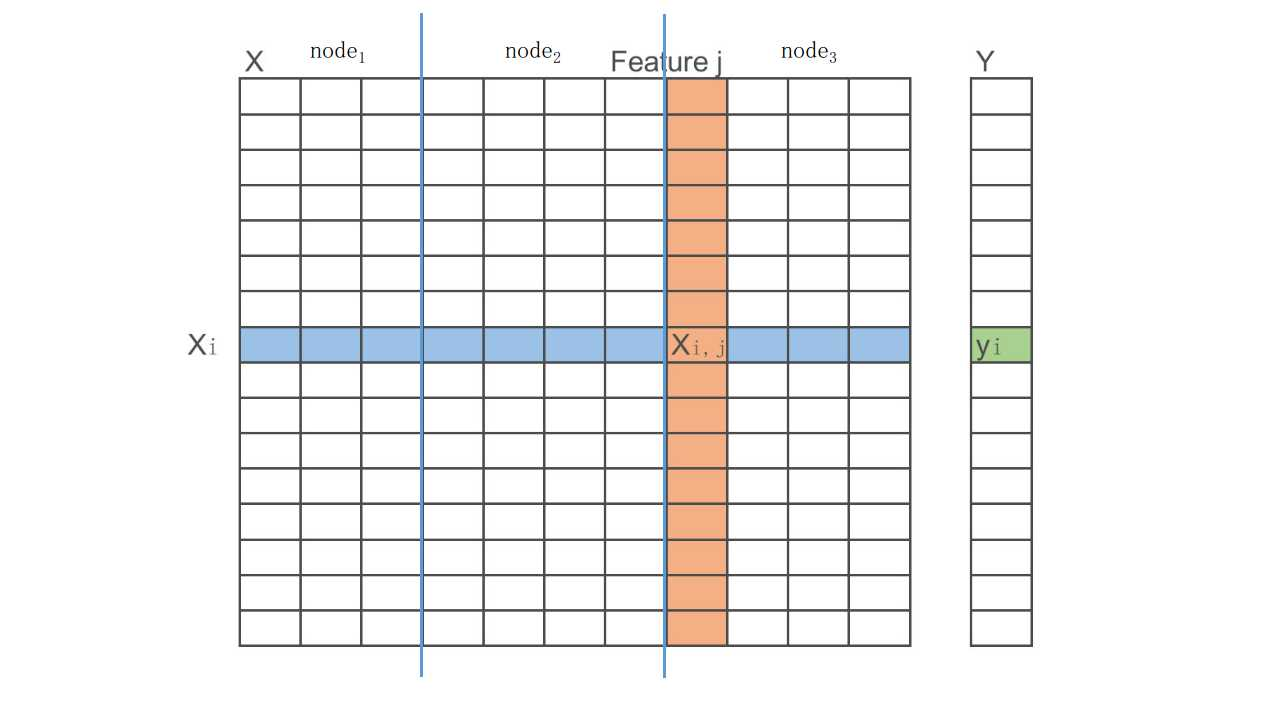
\includegraphics[width=.5\linewidth]{figs/datapartition2.jpg}
		\end{figure}
		

		\begin{itemize}
			\item Partition by rows (samples) 
			\begin{itemize}			
				\item need gobal communication to build \textcolor{red}{Bins}, once if use global static Bins.
				\item need gobal communication to build \textcolor{red}{GHSum} for each feature in findBestSplit() $\rightarrow$ \textcolor{blue}{allreduce(GHSum)}
			\end{itemize}			
			\item Partition by columns (features)
			\begin{itemize}			
				\item \textcolor{red}{Bins} and \textcolor{red}{GHSum} are all local, no communication
				\item need global communication to select the best feature in findBestSplit() $\rightarrow$ \textcolor{blue}{allreduce(maxscore)}
			\end{itemize}			
			
		\end{itemize}
	
\end{frame}

\begin{frame}
	\frametitle{Issue - Overhead of Synchronization \& Communication}
	%\textbf{Heading}
	\begin{itemize}
		\item Overhead of communication
		\begin{itemize}			
			\item well designed Bins works as model compression, reducing the data volume of communication
			\item pipeline 
		\end{itemize}			
		\item Overhead of synchronization
		\begin{itemize}			
			\item load imbalance is the killer of synchronization operation
			\item allreduce give chance to \textcolor{blue}{model rotation}
			\item stochastic GBT give chance to \textcolor{blue}{timer control} 
		\end{itemize}			
		
	\end{itemize}
	
\end{frame}

\section{Future Work} % Sections 
\subsection{Topics for the Next Step} 
\begin{frame}
	\frametitle{Topics for the Next Step}
	\begin{itemize}
		\item memory access optimization in shared memory system
		\item load imbalance issue in distributed system
		\item different Bins design
		\item dataset with sparsity and high dimensionality
	\end{itemize}
\end{frame}



%------------------------------------------------
%appendix

%------------------------------------------------

\begin{frame}
\frametitle{References}
%This statement requires citation \cite{p1}.
\footnotesize{
\begin{thebibliography}{99} % Beamer does not support BibTeX so references must be inserted manually as below
%\bibitem[Smith, 2012]{p1} John Smith (2012)
%\newblock Title of the publication
%\newblock \emph{Journal Name} 12(3), 45 -- 678.

\bibitem[Chen 2016]{Chen}T. Chen and C. Guestrin, “Xgboost: A scalable tree boosting system,” in Proceedings of the 22nd acm sigkdd international conference on knowledge discovery and data mining, 2016, pp. 785--794..

\bibitem[Tyree 2011]{Tyree}S. Tyree, K. Q. Weinberger, K. Agrawal, and J. Paykin, “Parallel boosted regression trees for web search ranking,” in Proceedings of the 20th international conference on World wide web, 2011, pp. 387--396.

\end{thebibliography}
}
\end{frame}



%------------------------------------------------

\begin{frame}
\Huge{\centerline{The End}}
\end{frame}

%----------------------------------------------------------------------------------------

\end{document} 
